% 手拉手 引入题：△OAB, △OCD 均等腰，∠AOB=∠COD=50°，求证 AC=BD
\documentclass[tikz,border=4pt]{standalone}
\usepackage{ctex}
\usepackage{amsmath}
\usetikzlibrary{calc, decorations.markings}
\begin{document}
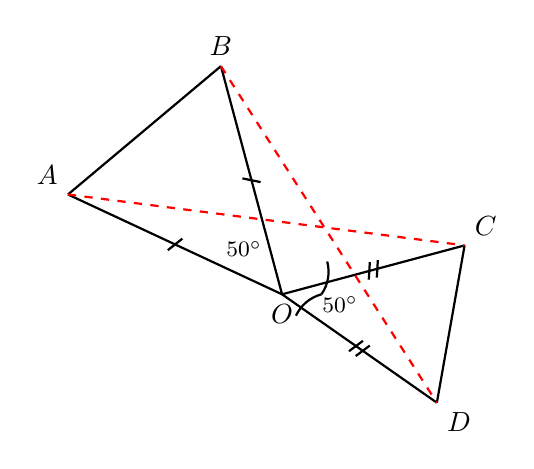
\begin{tikzpicture}[scale=1.0, thick,
  tick/.style={postaction={decorate, decoration={markings,
    mark=at position 0.5 with {\draw (-1.5pt,-3pt) -- (1.5pt,3pt);}}}},
  ticktwo/.style={postaction={decorate, decoration={markings,
    mark=at position 0.5 with {\draw (-2.5pt,-3pt) -- (-0.5pt,3pt);
                               \draw (0.5pt,-3pt)  -- (2.5pt,3pt);}}}}]
  \coordinate (O) at (0,0);
  % △OAB 顶角 50°，OA=OB=3，张角中线方向 130°
  \coordinate (A) at ({3*cos(155)}, {3*sin(155)});
  \coordinate (B) at ({3*cos(105)}, {3*sin(105)});
  % △OCD 顶角 50°，OC=OD=2.4，中线方向 -10°
  \coordinate (C) at ({2.4*cos(15)}, {2.4*sin(15)});
  \coordinate (D) at ({2.4*cos(-35)}, {2.4*sin(-35)});

  \draw[tick] (O) -- (A);
  \draw[tick] (O) -- (B);
  \draw (A) -- (B);
  \draw[ticktwo] (O) -- (C);
  \draw[ticktwo] (O) -- (D);
  \draw (C) -- (D);

  % 顶角弧
  \draw (0.5,0) ++(105:0) arc[start angle=105, end angle=155, radius=0.5];
  \node at ({0.75*cos(130)},{0.75*sin(130)}) {\footnotesize $50^\circ$};
  \draw (0.5,0) ++(-35:0) arc[start angle=-35, end angle=15, radius=0.5];
  \node at ({0.75*cos(-10)},{0.75*sin(-10)}) {\footnotesize $50^\circ$};

  \draw[red, dashed] (A) -- (C);
  \draw[red, dashed] (B) -- (D);

  \node[below]       at (O) {$O$};
  \node[above left]  at (A) {$A$};
  \node[above]       at (B) {$B$};
  \node[above right] at (C) {$C$};
  \node[below right] at (D) {$D$};
\end{tikzpicture}
\end{document}
